
\documentclass[oneside,a4paper]{book}
%\pagestyle{headings}


%=============================================================================

\usepackage{amsthm}
\usepackage{xspace}
\usepackage{float}
\usepackage{ifthen}
\usepackage{amsbsy}
\usepackage{amssymb}
\usepackage{balance}
\usepackage{booktabs}
\usepackage{graphicx}
\usepackage{rotating}
\usepackage{multirow}
\usepackage{needspace}
\usepackage{microtype}
\usepackage{bold-extra}
\usepackage{geometry}
\usepackage{varioref}
\usepackage{xcolor}
\usepackage{textcomp}
\usepackage{listings}
\usepackage[normalem]{ulem} %emphasize still italic
\usepackage{ucs}

% \usepackage[utf8]{inputenc}
% \usepackage[htt]{hyphenat}
\usepackage{times}
\usepackage{url}
\usepackage{alltt}
\usepackage{amsmath}
\usepackage{xfrac}
\usepackage{subfigure}
\usepackage{appendix}
\usepackage{stmaryrd}   % for the \shortuparrow
\usepackage[utopia]{quotchap}

\usepackage{setspace}
\usepackage[numbers, sort&compress]{natbib}
\usepackage{mdwlist}        % support for better spaced lists
% allows for temporary adjustment of side margins
\usepackage{chngpage}
\usepackage[normalem]{ulem}
\usepackage{dblfloatfix}

% constants

\newcounter{qcounter}

% commands
\newcommand{\n}{$\cdot$}
\newcommand{\y}{\checkmark}
\newcommand{\subscript}[1]{$_{\textrm{\footnotesize{#1}}}$}
\newcommand{\superscript}[1]{$^{\textrm{\footnotesize{#1}}}$}
\newcommand{\vertical}[1]{\raisebox{-4em}{\begin{sideways}{#1}\end{sideways}}}

\newboolean{showedits}
\setboolean{showedits}{true} % toggle to show or hide edits
\ifthenelse{\boolean{showedits}}
{
       \newcommand{\ugh}[1]{\textcolor{red}{\uwave{#1}}} % please rephrase
       \newcommand{\ins}[1]{\textcolor{blue}{\uline{#1}}} % please insert
       \newcommand{\del}[1]{\textcolor{red}{\sout{#1}}} % please delete
       \newcommand{\chg}[2]{\textcolor{red}{\sout{#1}}{\ra}\textcolor{blue}{\uline{#2}}} % please change
}{
       \newcommand{\ugh}[1]{#1} % please rephrase
       \newcommand{\ins}[1]{#1} % please insert
       \newcommand{\del}[1]{} % please delete
       \newcommand{\chg}[2]{#2}
}


% ============================================================================
% Put edit comments in a really ugly standout display

\usepackage{xcolor}
\usepackage[normalem]{ulem}
\newcommand{\ra}{$\rightarrow$}


% comments \nb{label}{color}{text}
\newboolean{showcomments}
\setboolean{showcomments}{true}
\ifthenelse{\boolean{showcomments}}
    {\newcommand{\nb}[3]{
        {\colorbox{#2}{\bfseries\sffamily\scriptsize\textcolor{white}{#1}}}
        {\textcolor{#2}{\sf\small$\blacktriangleright$\textit{#3}$\blacktriangleleft$}}}
     \newcommand{\version}{\emph{\scriptsize$-$Id$-$}}
%	 \newcommand{\ugh}[1]{\textcolor{red}{\uwave{#1}}} % please rephrase
%	 \newcommand{\ins}[1]{\textcolor{blue}{\uline{#1}}} % please insert
%	 \newcommand{\del}[1]{\textcolor{red}{\sout{#1}}} % please delete
%	 \newcommand{\chg}[2]{\textcolor{red}{\sout{#1}}{\ra}\textcolor{blue}{\uline{#2}}} % please change
	 \newcommand{\chk}[1]{\textcolor{ForestGreen}{#1}} % changed, please check
	}
    {\newcommand{\nb}[3]{}
     \newcommand{\version}{}
	\newcommand{\chk}[1]{} % changed, please check
	}

% ============================================================================
% Make quotes be italic
\renewenvironment{quote}
    {\list{}{\rightmargin\leftmargin}%
     \item\relax\begin{it}}
    {\end{it}\endlist}

\newcommand{\ttimes}{\ensuremath{\times}}

%=============================================================================

\newcommand{\needlines}[1]{\Needspace{#1\baselineskip}}

% source code
\usepackage{xcolor}
\usepackage{textcomp}
\usepackage{listings}
\definecolor{source}{gray}{0.9}
\lstset{
	language={},
	% characters
	tabsize=3,
	upquote=true,
	escapechar={!},
	keepspaces=true,
	breaklines=false,
	alsoletter={:},
	breakautoindent=true,
	columns=fullflexible,
	showstringspaces=false,
	basicstyle=\footnotesize\ttfamily,
	% background
	frame=single,
    framerule=0pt,
	backgroundcolor=\color{source},
	% numbering
	numbersep=5pt,
	numberstyle=\tiny,
	numberfirstline=true,
	% captioning
	captionpos=b,
	numberbychapter=false,
	% formatting (html)
	moredelim=[is][\textbf]{<b>}{</b>},
	moredelim=[is][\textit]{<i>}{</i>},
	moredelim=[is][\uline]{<u>}{</u>}}
\newcommand{\ct}{\lstinline[backgroundcolor=\color{white},basicstyle=\footnotesize\ttfamily]}
\newcommand{\lct}[1]{{\small\tt #1}}


%----------------------------------------------------------------------------
% references
\newcommand{\tabref}[1]{\hyperref[{tab:#1}]{Table~\ref*{tab:#1}}}
\newcommand{\figref}[1]{\hyperref[{fig:#1}]{Figure~\ref*{fig:#1}}}
\newcommand{\secref}[1]{\hyperref[{sec:#1}]{Section~\ref*{sec:#1}}}
\newcommand{\lstref}[1]{\hyperref[{lst:#1}]{Listing~\ref*{lst:#1}}}
\newcommand{\charef}[1]{\hyperref[{cha:#1}]{Chapter~\ref*{cha:#1}}}
%----------------------------------------------------------------------------

% abbreviations
\tracingcolors 4
\setcounter{tocdepth}{3}
\setcounter{secnumdepth}{3}
\newcommand{\ie}{\emph{i.e.,}\xspace}
\newcommand{\eg}{\emph{e.g.,}\xspace}
\newcommand{\etc}{\emph{etc.}\xspace}
\newcommand{\etal}{\emph{et al.}\xspace}


\newcommand{\newevenside}{
	\ifthenelse{\isodd{\thepage}}{\newpage}{
	\newpage
        \phantom{placeholder} % doesn't appear on page
	\thispagestyle{empty} % if want no header/footer
	\newpage
	}
}

\def\stretchfactor{1}
\newcommand{\mychapter}[1]{\setstretch{1}
    \chapter{#1}\setstretch{\stretchfactor}}

%----------------------------------------------------------------------------
\newcommand{\lessSpace}{\vspace{-1em}}
\DeclareGraphicsExtensions{.pdf,.png}
\graphicspath{{images/}}
\newcommand{\fig}[4]{
	\begin{figure}[#1]
		\centering
		\includegraphics[width=#2\textwidth]{#3}
		\lessSpace
		\caption{\label{fig:#3}#4}
	\end{figure}}

% ===========================================================================


\newcommand{\thesistitle}{Deep Reinforcement Learning Othello}
\newcommand{\thesisauthor}{Thomas Steinmann}
\newcommand{\thesisleiter}{Paolo Favaro}
\newcommand{\thesisasst}{}
\newcommand{\thesissubtitle}{Thesis subtitle}
\newcommand{\thesisdate}{Month and Year}



% ===========================================================================

\usepackage[ colorlinks=true, urlcolor=black, linkcolor=black,
			citecolor=black, bookmarksnumbered=true, bookmarks=true,
			plainpages=false,
			pdftitle={\thesistitle}, pdfauthor={\thesisauthor},
			pdfsubject={\thesissubtitle}, pdfpagelabels]{hyperref}

\newcommand{\hrref}[2]{\hyperref}
% ===========================================================================
% ===========================================================================


% D O C U M E N T
% % % % % % % % % % % % % % % % % % % % % % % % % % % % % % % % % %
\begin{document}

% T I T L E
% % % % % % % % % % % % % % % % % % % % % % % % % % % % % % % % % %
\begin{titlepage}  
  \begin{center}  
  
  \begin{figure}[t]  
  \vspace*{-2cm}        % to move header logo at the top 
  \center{
\includegraphics[scale=0.2]{logos/MSc_quer.png}}
  \vspace{0.4in}     
  \end{figure}

    \thispagestyle{empty}
    
    {\bfseries\Huge \thesistitle \par
    \Large \vspace{0.1in} \thesissubtitle \par}

    \vspace{0.3in} 
    \LARGE{\textbf{Master Thesis} \\}
    \vspace{0.4in}

    {\Large \thesisauthor}
    
    \vspace{0.3in}
    {\Large University of Bern \par}
%    {\Large Philosophisch-naturwissenschaftlichen Fakult\"{a}t \\
%            der Universit\"{a}t Bern \par}
    \vfill
    {\Large \thesisdate \par}
  

  \vspace{0.9in}
 
  % === Logos ==============================================     
  \begin{figure}[htp]
    \centering
    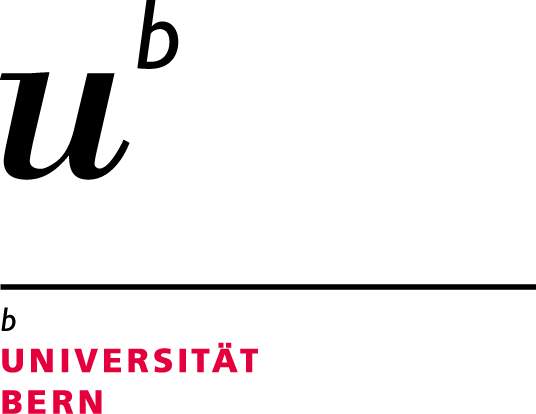
\includegraphics[scale=0.30]{logos/UNI_Bern.png}\hfill
    
\includegraphics[scale=0.30]{logos/UNI_Neuenburg.png}\hfill
    
\includegraphics[scale=0.80]{logos/UNI_Fribourg.png}
  \end{figure}
  % === // Logos ===========================================    


  \end{center}

\end{titlepage}

\graphicspath{{images/}}

% A B S T R A C T
% % % % % % % % % % % % % % % % % % % % % % % % % % % % % % % % % %
\chapter*{\centering Abstract}
\begin{quotation}
\noindent 
Abstract (max. 1 page)

Name of the Supervisor, Group, Institute, University, Supervisor

Name of the Assistant, Group, Institute, University, Assistant
\end{quotation}
\clearpage


% C O N T E N T S 
% % % % % % % % % % % % % % % % % % % % % % % % % % % % % % % % % % % % % % % %
\tableofcontents

%%%%%%%% Introduction %%%%%%%%
\chapter {Introduction}
\label {cha:introduction}
With recent successes such as AlphaGo defeating the reigning world champion and fast progress towards fully autonomous cars by Tesla as well as Weymo it is clear that Reinforcement Learning is the solution to many problems that could not even be tackled before. Many of these powerful implementations rely on equally powerful machines in order to train them, often requiring over hundred CPUs and GPUs for weeks on end. Inspired by these grand achievements and the technology behind them but lacking comparable resources I settled on a more achievable goal: Othello. This simple board game has accompanied me since the first semester when we were tasked to implement a search based Othello player. During my masters studies I suspected that a superior player could be created using machine learning techniques. This thesis documents the way to such a player and its key components.


%%%%%%%% Related Works %%%%%%%%
\chapter {Related Works}
\label {cha:Related Works}

\section {Othello}
\label{sec:Othello}

\begin{figure}[!b]
  \centering
	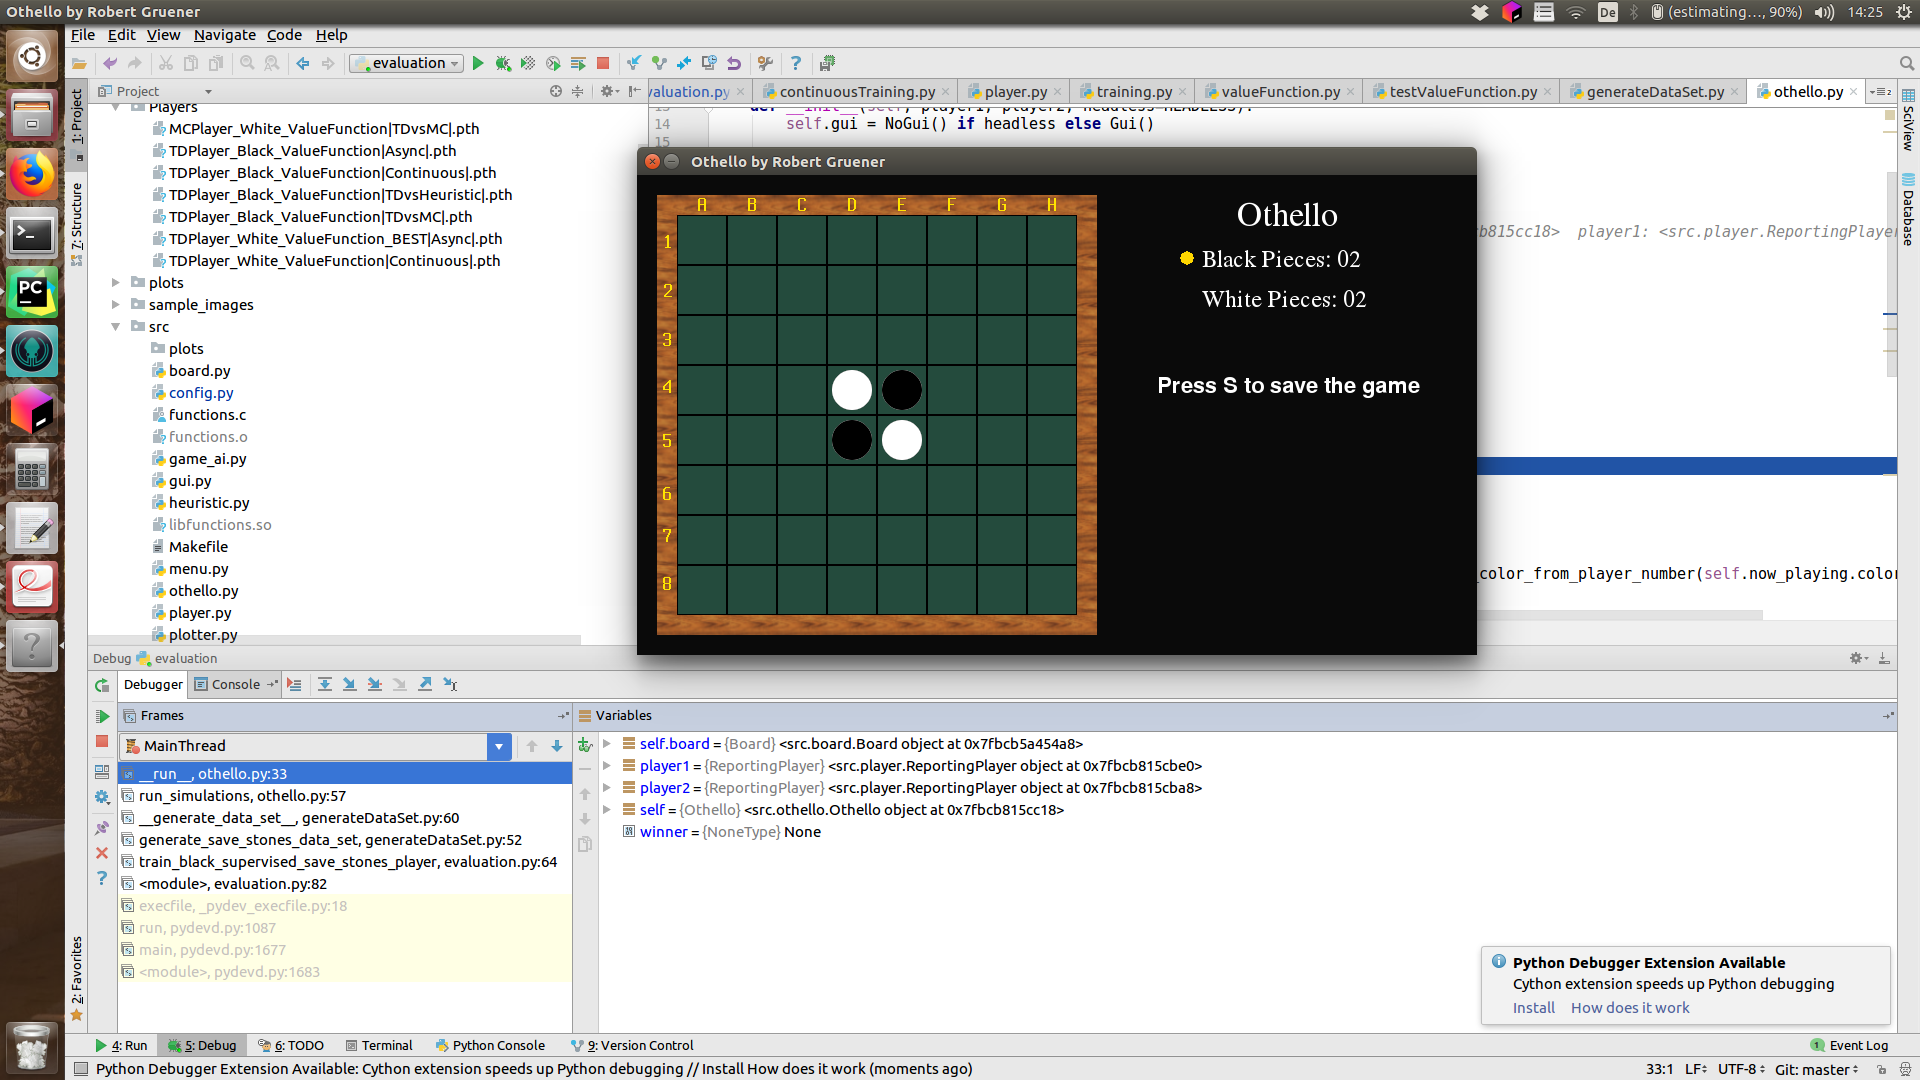
\includegraphics[scale=0.5]{OpeningPosition.png}
	\caption{The opening position}
	\label{fig:OpeningPosition}
\end{figure}

According to \cite{RULES} Othello is a game played on a  square board, usually made up of eight by eight tiles.
The opening position is shown in Figure \ref{fig:OpeningPosition}
Othello stones are black on one side and white on the other. Players take turns in placing one of these stones in their respective color on the board. Stones can only be placed in such a way that the new stone \textit{traps} one or more of the opponents stones inbetween itself and any other stone of the same color. All opposing stones that were trapped by placing the new stone are flipped and now belong to the player who trapped them. If a player cannot perform a legal move he simply passed and his opponent places the next stone. The game ends if both players pass successively or there are no free tiles left on the board. The player who controls more stones at this time wins the game.

\section {Heuristic Player}
\label{sec:Heuristic Player}
The player we call the \textit{Heuristic} Player in this thesis is often used for benchmarking because of its decent performance, low computational cost and deterministic nature. It utilises a heuristic table which assigns a value to each tile on the board. These values are symmetrical for eight axes through the board. The table gives high values to tiles such as the edges that are of high value because they lead to stones that cannot be captured later in the game. Tiles around the edges however receive a low value because occupying one of them may allow the opponent to occupy the adjacent corner.

\section {Search based Algorithms}
\label{sec:Search based Algorithms}
Othello is widely used to teach search based game theory algorithms, most notably the min-max algorithm and its optimization the alpha-beta pruning. \cite{AI} The general idea of these methods is to build a search tree of all relevant moves for both players and the resulting game states. Ideally a complete graph for such a game could be computed and a computer player would just choose a move that results in a win for every single turn. However the search space for most games is so big that such a graph is not feasible with the computational resources available. The ancient chinese game of Go for example is said to have more possible game states than there are atoms in the universe. The challenge lies therefore in approximating a complete graph as close as possible and with maximal efficiency. For this the search tree is usually truncated at a certain depth or after a given time has passed and the rest of the tree is approximated with a so called value function that evaluates the value of the state where the tree stopped. This value function traditionally consists of a set of given features such as possible moves for each player, save stones that cannot be captured again or just greedily the number of stones a player controls. Search based algorithms can also be used to improve the \textit{Heuristic Player} described in section \ref{sec:Heuristic Player}. In most search based algorithms this would make the player nondeterministic however.

\section {Machine Learning based Algorithms}
\label{sec:Machine Learning based Algorithms}
Machine learning techniques for Othello are related to search based algorithms but often do not perform a search at play time. A straight forward approach is to inprove a search based algorithm by learning its value function. \cite{CHERRY} used machine learning to learn his own heuristics function, similar to the one used by the \textit{Heuristic Player}, in his alpha-beta search algorithm. A more advanced technique basically moves the search from play time to training time by simulating thousands or millions of games and uses them to train an agent. This agent learns a value function that captures the knowledge gained during the search and predicts the value of a possible move without having to perform another search at play time. Such an approach was used by \cite{DEEPMIND} to master Go. They went one step further still and used training time search in order to train an agent and then improved that agents decision again with another search at play time.

\section {Reinforcement Learning}
\label{sec:Reinforcement Learning}
Reinforcement Learning levarages special algorithms to train an agent on a task while performing it. In regular intervals the agent receives feedback, reinforcing behaviour that leads to good results while discouraging less performant ones. This is handled by awarding a positive or negative reward respectively, whenever the algorithm can determine something good or bad happened based on the agent's actions.

\subsection {Monte Carlo Learning}
\label{sec:Monte Carlo Learning}
Monte Carlo Learning is the most basic variant of a group of reinforcement learning algorithms called Monte Carlo Methods. In contrast to many other reinforcement learning algorithms they do not require full knowledge of the environment that they are applied o. Instead they work on experience alone. This experience can be gathered in the real environment and learning can therefore be done on the fly, without any prior knowledge. Another very powerful approach is to simulate the environment which allows for simpler aggregation of training data that would be difficult to obtain in the real world, such as driving cars, steering rockets or playing millions of board game iterations on a physical board.

In Monte Carlo Methods a task can be split in two major parts. First the reinforcement algorithm which is generating training data from real or simulated experience and an according label. Second a supervised learning task where an agent is trained on the data generated from the first part. Those two parts are mostly independent of each other, as long as the structure of in and outputs match. This means that the same reinforcement algorithm can be used with a variety of different learning agents such as, in the case of this thesis, multiple different neural networks.

The basic Monte Carlo Algorithm simply simulates an entire episode, evaluates the final state and labels each training sample with the resulting label. In a board game this would mean playing a single game, computing the winner and labeling the game state for each time step with the final result.

\subsection {Temporal Difference Learning }
\label{sec:Temporal difference Learning}
The Temporal Difference algorithm is a variant of the basic Monte Carlo algorithm decribed above. In contrast to its predecessor it does not assign the same label to each game state but rather computes each label based on the prediction of the subsequent state's value. This can be better understood when analysing the algorithm from the end of an episode. The final label is still the result of the game just like in the basic Monte Carlo algorithm. \ugh{check this again}The label of the second to last game state however is computed from its current value as well as the value of the final state. This allows for a so called online version of the algorithm which does not have to complete an entire episode before it can learn from the gathered experience, but can apply changes at every time step of the episode. Although the online version has weaker convergence guarantees and since standard Othello episodes have a maximum length of 30 game states per player there is a guaranteed reward in relatively few time steps which makes offline Temporal Difference Learning more suitable for this thesis.

\subsection {Monte Carlo Tree Search}
\label{sec:Monte Carlo Tree Search}

%%%%%%%% Thesis Objectives %%%%%%%%
\chapter {Thesis Objectives}
\label{cha:Thesis Objectives}
1. Framwork for othello agents
2. Playground for RL algorithms, network optimizations, regularizations, etc.
3. High performance Othello Agent

\section {Othello}
\label{sec:Othello}
One of the main difficulties in applying reinforcement learning to Othello is the very delayed and sparse reward. The only evaluation the learning algorithm can make is the result of the game, every other measure would introduce prior knowledge and therefore influence the strategy that is learned by the player. This constrains the learning algorithm to a single reward per game, rather than one for every action taken like for example in a jump and run game.


%%%%%%%% Implementation %%%%%%%%
\chapter {Implementation}
\label{cha:Implementation}

%%%%%%%% Validation %%%%%%%%
\chapter {Validation}
\label{cha:Validation}

%%%%%%%% Conclusion %%%%%%%%
\chapter {Conclusion}
\label{cha:Conclusion}

%%%%%%%% Future Work %%%%%%%%
\chapter {Future Work}
\label{cha:Future Work}


%END Doc
%-------------------------------------------------------

\bibliographystyle{plain}
\bibliography{Thesis}

\end{document}
